\documentclass[12pt,a4paper]{article}
\usepackage[utf8]{vietnam}
\usepackage{amsmath,amssymb}
\usepackage{tabularx}
\usepackage{tikz}
\usetikzlibrary{calc,angles,quotes,arrows.meta}
\usepackage{xcolor}
\usepackage{enumitem}
\usepackage{fancyhdr}
\usepackage[top=1.0cm, bottom=1.1cm, left=1.3cm, right=1.3cm]{geometry}
\usepackage[dethi]{ex_test}
\SAOPTN{widthSA=3.2,heightSA=0.62}

\setlength{\headheight}{15pt}
\setlength{\parskip}{1.5pt}

\pagestyle{fancy}
\fancyhf{}
\lhead{\textit{Trường THCS Sơn Tây -- Hướng dẫn giải Đề KSCL Lớp 9 Lần 1}}
\rhead{\textit{Năm học 2026 -- 2027 | Môn Toán (Mã đề: 02)}}
\cfoot{\thepage/4}

\begin{document}

% =============================================================================
% TRANG 1: TIÊU ĐỀ & PHẦN I TRẮC NGHIỆM
% =============================================================================
\begin{center}
  {\bfseries\large TRƯỜNG THCS SƠN TÂY \hfill ĐỀ KHẢO SÁT CHẤT LƯỢNG LỚP 9 -- LẦN 1}\\
  \vspace{1mm}
  {\bfseries\Large HƯỚNG DẪN GIẢI CHI TIẾT VÀ BAREM THANG ĐIỂM}\\
  \vspace{1mm}
  \textit{Năm học 2026 -- 2027 | Môn: TOÁN (MÃ ĐỀ: 02) | Thời gian làm bài: 90 phút}
\end{center}
\vspace{-1.5mm}
\hrule
\vspace{2.5mm}

\noindent\textbf{\large I. PHẦN TRẮC NGHIỆM (2,0 điểm)}

\textit{Mỗi câu trả lời đúng được 0,25 điểm.}

\begin{center}
\begin{tabular}{|c|c|c|c|c|c|c|c|c|}
\hline
\textbf{Câu} & \textbf{1} & \textbf{2} & \textbf{3} & \textbf{4} & \textbf{5} & \textbf{6} & \textbf{7} & \textbf{8} \\
\hline
\textbf{Đáp án} & \textbf{B} & \textbf{D} & \textbf{A} & \textbf{C} & \textbf{D} & \textbf{C} & \textbf{A} & \textbf{C} \\
\hline
\end{tabular}
\end{center}
\vspace{1.5mm}

\noindent\textbf{Giải thích chi tiết phương án chọn:}
\begin{itemize}[leftmargin=18pt, itemsep=3.5pt, parsep=0pt]
  \item \textbf{Câu 1 (Chọn B):} Phương trình bậc nhất hai ẩn có dạng $ax + by = c$ ($a, b$ không đồng thời bằng 0; các ẩn $x, y$ có số mũ là 1). Do đó $3x + y = 0$ là phương trình bậc nhất hai ẩn.
  \item \textbf{Câu 2 (Chọn D):} $3x + 4 = 1 \iff 3x = 1 - 4 \iff 3x = -3 \iff x = -1$.
  \item \textbf{Câu 3 (Chọn A):} Thay $(x; y) = (2; 1)$ vào phương trình $x + 3y = 5$, ta có $2 + 3(1) = 5$ (đúng).
  \item \textbf{Câu 4 (Chọn C):} Thay cặp số $(-2; 3)$ vào hệ phương trình ở phương án C:
  \[
    \begin{cases}
      -2 + 3 = 1 \text{ (đúng)} \\
      -2 - 3(3) = -2 - 9 = -11 \text{ (đúng)}
    \end{cases}
  \]
  Vậy $(-2; 3)$ là nghiệm của hệ phương trình ở phương án C.
  \item \textbf{Câu 5 (Chọn D):} $x + 6 \le 0 \iff x \le -6$.
  \item \textbf{Câu 6 (Chọn C):} Cho đường tròn $(O; R)$, điểm $M$ nằm bên trong đường tròn khi và chỉ khi khoảng cách từ $M$ đến tâm $O$ nhỏ hơn bán kính: $OM < R$.
  \item \textbf{Câu 7 (Chọn A):} Trong tam giác $ABC$ vuông tại $A$, cạnh đối của góc $C$ là $AB$, cạnh huyền là $BC$. Do đó $\sin C = \dfrac{AB}{BC}$.
  \item \textbf{Câu 8 (Chọn C):} Trong tam giác $ABC$ vuông tại $A$:\\
  $\tan C = \dfrac{AB}{AC} = \dfrac{3\sqrt{3}}{3} = \sqrt{3} \implies \widehat{C} = 60^\circ$.
\end{itemize}

\newpage

% =============================================================================
% TRANG 2: CÂU 9, CÂU 10 & CÂU 11
% =============================================================================
\noindent\textbf{\large II. PHẦN TỰ LUẬN (8,0 điểm)}

\vspace{1.5mm}
\noindent\textbf{Câu 9 (2,0 điểm).} Giải các phương trình sau:

\begin{enumerate}[label=\alph*), leftmargin=18pt, itemsep=3pt, parsep=0pt]
  \item $(2 - x)(2x + 1) = 0$ \hfill \textbf{(1,0 điểm)}
  \begin{itemize}[leftmargin=16pt, itemsep=1.5pt, parsep=0pt]
    \item Đưa về hai trường hợp: $\left[\begin{aligned} 2 - x &= 0 \\ 2x + 1 &= 0 \end{aligned}\right.$ \dotfill \textbf{0,50 điểm}
    \item Giải tìm $x$: $\left[\begin{aligned} x &= 2 \\ 2x &= -1 \end{aligned}\right. \iff \left[\begin{aligned} x &= 2 \\ x &= -\dfrac{1}{2} \end{aligned}\right.$ \dotfill \textbf{0,25 điểm}
    \item Kết luận: Vậy tập nghiệm của phương trình là $S = \left\{-\dfrac{1}{2}; 2\right\}$. \dotfill \textbf{0,25 điểm}
  \end{itemize}

  \item $\dfrac{3}{x + 1} + \dfrac{2}{x - 3} = \dfrac{3}{(x + 1)(x - 3)}$ \hfill \textbf{(1,0 điểm)}
  \begin{itemize}[leftmargin=16pt, itemsep=1.5pt, parsep=0pt]
    \item Điều kiện xác định: $\begin{cases} x + 1 \neq 0 \\ x - 3 \neq 0 \end{cases} \iff \begin{cases} x \neq -1 \\ x \neq 3 \end{cases}$. \dotfill \textbf{0,25 điểm}
    \item Quy đồng mẫu và khử mẫu:
    $3(x - 3) + 2(x + 1) = 3$ \dotfill \textbf{0,25 điểm}
    \item Khai triển và thu gọn:
    $3x - 9 + 2x + 2 = 3 \iff 5x - 7 = 3 \iff 5x = 10 \iff x = 2$. \dotfill \textbf{0,25 điểm}
    \item Đối chiếu ĐKXĐ: $x = 2$ thỏa mãn điều kiện. Vậy nghiệm là $x = 2$. \dotfill \textbf{0,25 điểm}
  \end{itemize}
\end{enumerate}

\vspace{2mm}
\hrule
\vspace{2mm}

\noindent\textbf{Câu 10 (1,0 điểm).} Giải hệ phương trình: $\begin{cases} x + 5y = -11 \\ 2x - 3y = 4 \end{cases}$
\begin{itemize}[leftmargin=16pt, itemsep=1.5pt, parsep=0pt]
  \item Từ phương trình thứ nhất suy ra: $x = -11 - 5y$. \dotfill \textbf{0,25 điểm}
  \item Thế vào phương trình thứ hai:
  $2(-11 - 5y) - 3y = 4 \iff -22 - 10y - 3y = 4 \iff -13y = 26 \iff y = -2$. \dotfill \textbf{0,25 điểm}
  \item Thay $y = -2$ vào biểu thức của $x$: $x = -11 - 5(-2) = -11 + 10 = -1$. \dotfill \textbf{0,25 điểm}
  \item Kết luận: Vậy hệ phương trình có nghiệm duy nhất $(x; y) = (-1; -2)$. \dotfill \textbf{0,25 điểm}
\end{itemize}

\vspace{2mm}
\hrule
\vspace{2mm}

\noindent\textbf{Câu 11 (1,0 điểm).} \textit{Giải bài toán bằng cách lập hệ phương trình:}
\begin{itemize}[leftmargin=16pt, itemsep=1.5pt, parsep=0pt]
  \item Gọi số thí sinh dự thi của trường A là $x$ (thí sinh, điều kiện: $x \in \mathbb{N}^*, x < 385$).\\
  Gọi số thí sinh dự thi của trường B là $y$ (thí sinh, điều kiện: $y \in \mathbb{N}^*, y < 385$). \dotfill \textbf{0,25 điểm}
  \item Tổng số học sinh dự thi là 385 nên ta có phương trình: $x + y = 385 \quad (1)$. \dotfill \textbf{0,25 điểm}
  \item Số học sinh trúng tuyển trường A là $90\%x = 0{,}9x$; trường B là $80\%y = 0{,}8y$.\\
  Tổng số học sinh trúng tuyển là 327 nên có phương trình: $0{,}9x + 0{,}8y = 327 \quad (2)$. \dotfill \textbf{0,25 điểm}
  \item Giải hệ phương trình:
  \[
    \begin{cases}
      x + y = 385 \\
      0{,}9x + 0{,}8y = 327
    \end{cases}
    \iff
    \begin{cases}
      0{,}8x + 0{,}8y = 308 \\
      0{,}9x + 0{,}8y = 327
    \end{cases}
    \iff
    \begin{cases}
      0{,}1x = 19 \\
      y = 385 - x
    \end{cases}
    \iff
    \begin{cases}
      x = 190 \\
      y = 195
    \end{cases}
    \text{ (TMĐK)}.
  \]
  Vậy trường A có 190 thí sinh dự thi, trường B có 195 thí sinh dự thi. \dotfill \textbf{0,25 điểm}
\end{itemize}

\newpage

% =============================================================================
% TRANG 3: CÂU 12 & CÂU 13
% =============================================================================
\noindent\textbf{Câu 12 (1,0 điểm).}
\par\noindent
\begin{minipage}[t]{0.70\linewidth}
Một cái cây có bóng trên mặt đất dài $40\,\text{m}$, biết rằng góc tạo bởi tia nắng mặt trời với mặt đất là $35^\circ$. Hỏi cái cây cao bao nhiêu mét? (làm tròn đến mét).

\vspace{1.5mm}
\noindent\textbf{Lời giải chi tiết:}
\begin{itemize}[leftmargin=14pt, itemsep=1.5pt, parsep=0pt]
  \item Mô hình hóa: Thân cây thẳng đứng $AC$ vuông góc với mặt đất tại $C$, bóng cây trên mặt đất là $BC = 40\,\text{m}$, góc tạo bởi tia nắng mặt trời và mặt đất là $\widehat{ABC} = 35^\circ$. \dotfill \textbf{0,25 điểm}
  \item Tam giác $ABC$ vuông tại $C$, áp dụng tỉ số lượng giác góc nhọn:
  \[
    \tan B = \frac{AC}{BC} \implies AC = BC \cdot \tan 35^\circ
  \] \dotfill \textbf{0,25 điểm}
  \item Tính toán: $AC = 40 \cdot \tan 35^\circ \approx 40 \cdot 0{,}7002 = 28{,}008\,\text{m}$. \dotfill \textbf{0,25 điểm}
  \item Kết luận: Vậy cái cây cao khoảng $28\,\text{m}$. \dotfill \textbf{0,25 điểm}
\end{itemize}
\end{minipage}\hfill
\begin{minipage}[t]{0.28\linewidth}
\vspace{-2mm}
\centering
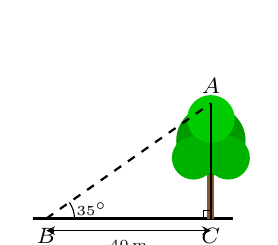
\begin{tikzpicture}[scale=0.55, >=stealth]
  \draw[thick] (-0.3,0) -- (4.3,0);
  \coordinate (C) at (3.8,0);
  \coordinate (B) at (0,0);
  \coordinate (A) at (3.8,2.66);
  
  \node[below] at (B) {\footnotesize $B$};
  \node[below] at (C) {\footnotesize $C$};
  \node[above] at (A) {\footnotesize $A$};
  
  % Thân cây và tán cây
  \draw[brown!70!black, line width=2.5pt] (3.8,0) -- (3.8,1.2);
  \fill[green!60!black] (3.8,1.8) circle (0.8);
  \fill[green!70!black] (3.4,1.4) circle (0.5);
  \fill[green!70!black] (4.2,1.4) circle (0.5);
  \fill[green!80!black] (3.8,2.3) circle (0.55);
  \draw[line width=1.0pt] (3.8,0) -- (3.8,2.66);
  
  % Tia nắng
  \draw[thick, dashed] (B) -- (A);
  
  % Góc vuông tại C
  \draw (C) ++(0,0.18) -- ++(-0.18,0) -- ++(0,-0.18);
  
  % Góc 35 độ tại B
  \draw (B) ++(0.65,0) arc (0:35:0.65);
  \node at (1.05,0.22) {\tiny $35^\circ$};
  
  \draw[<->] (0,-0.28) -- (3.8,-0.28);
  \node[below] at (1.9,-0.28) {\tiny $40\,\text{m}$};
\end{tikzpicture}
\end{minipage}

\vspace{2mm}
\hrule
\vspace{2mm}

\noindent\textbf{Câu 13 (2,0 điểm).}
\par\noindent
\begin{minipage}[t]{0.70\linewidth}
Cho $\Delta ABC$ vuông tại $A$, đường cao $AH$ ($H \in BC$), $AB = 6\,\text{cm}, AC = 8\,\text{cm}$.
\begin{enumerate}[label=\alph*), leftmargin=16pt, itemsep=2pt, parsep=0pt]
  \item \textbf{(1,0 điểm)} Tính $BC, AH$ và số đo góc $B$ (làm tròn đến độ):
  \begin{itemize}[leftmargin=12pt, itemsep=1pt, parsep=0pt]
    \item Áp dụng định lí Pythagore trong $\Delta ABC$ vuông tại $A$:\\
    $BC = \sqrt{AB^2 + AC^2} = \sqrt{6^2 + 8^2} = 10\,\text{cm}$. \dotfill \textbf{0,25 điểm}
    \item Áp dụng hệ thức lượng $AH \cdot BC = AB \cdot AC$:\\
    $AH = \dfrac{AB \cdot AC}{BC} = \dfrac{6 \cdot 8}{10} = 4{,}8\,\text{cm}$. \dotfill \textbf{0,50 điểm}
    \item Tính số đo góc $B$:\\
    $\sin B = \dfrac{AC}{BC} = \dfrac{8}{10} = 0{,}8 \implies \widehat{B} \approx 53^\circ$. \dotfill \textbf{0,25 điểm}
  \end{itemize}
\end{enumerate}
\end{minipage}\hfill
\begin{minipage}[t]{0.28\linewidth}
\vspace{-2mm}
\centering
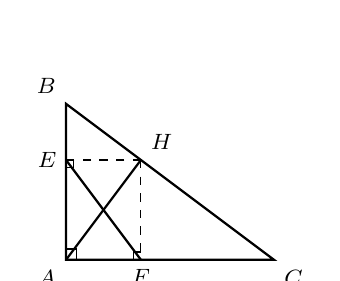
\begin{tikzpicture}[scale=0.55, >=stealth]
  \coordinate (A) at (0,0);
  \coordinate (B) at (0,3.6);
  \coordinate (C) at (4.8,0);
  
  \draw[thick] (A) node[below left]{\footnotesize $A$} 
            -- (B) node[above left]{\footnotesize $B$} 
            -- (C) node[below right]{\footnotesize $C$} -- cycle;
            
  \draw (0,0.25) -- (0.25,0.25) -- (0.25,0);
  
  \coordinate (H) at (1.728, 2.304);
  \draw[thick] (A) -- (H) node[above right]{\footnotesize $H$};
  
  \coordinate (E) at (0, 2.304);
  \coordinate (F) at (1.728, 0);
  \draw[dashed] (H) -- (E) node[left]{\footnotesize $E$};
  \draw[dashed] (H) -- (F) node[below]{\footnotesize $F$};
  \draw[thick] (E) -- (F);
  
  \draw (E) ++(0.18,0) -- ++(0,-0.18) -- ++(-0.18,0);
  \draw (F) ++(0,0.18) -- ++(-0.18,0) -- ++(0,-0.18);
\end{tikzpicture}
\end{minipage}

\begin{enumerate}[label=\alph*), leftmargin=16pt, itemsep=2pt, parsep=0pt, start=2]
  \item \textbf{(1,0 điểm)} Gọi $E, F$ là hình chiếu của $H$ trên $AB$ và $AC$. Chứng minh $AE \cdot AB = AF \cdot AC$ và $\Delta AEF \backsim \Delta ACB$:
  \begin{itemize}[leftmargin=16pt, itemsep=1.5pt, parsep=0pt]
    \item Xét $\Delta AHB$ vuông tại $H$, đường cao $HE$: $AH^2 = AE \cdot AB$ (hệ thức lượng). \dotfill \textbf{0,25 điểm}
    \item Xét $\Delta AHC$ vuông tại $H$, đường cao $HF$: $AH^2 = AF \cdot AC$ (hệ thức lượng). \dotfill \textbf{0,25 điểm}
    \item Suy ra: $AE \cdot AB = AF \cdot AC$ (vì cùng bằng $AH^2$). \dotfill \textbf{0,25 điểm}
    \item Từ $AE \cdot AB = AF \cdot AC \implies \dfrac{AE}{AC} = \dfrac{AF}{AB}$.\\
    Xét $\Delta AEF$ và $\Delta ACB$ có: $\widehat{A}$ chung và $\dfrac{AE}{AC} = \dfrac{AF}{AB}$.\\
    Do đó $\Delta AEF \backsim \Delta ACB$ (c-g-c) (đpcm). \dotfill \textbf{0,25 điểm}
  \end{itemize}
\end{enumerate}

\newpage

% =============================================================================
% TRANG 4: CÂU 14 & BẢNG MA TRẬN ĐIỂM
% =============================================================================
\noindent\textbf{Câu 14 (1,0 điểm).}
\begin{enumerate}[label=\alph*), leftmargin=18pt, itemsep=2.5pt, parsep=0pt]
  \item \textbf{(0,5 điểm)}
  \par\noindent
  \begin{minipage}[t]{0.72\linewidth}
    Xác định vị trí điểm $E$ trên cạnh $AB$ để diện tích vườn hoa $EFGH$ nhỏ nhất:
    \begin{itemize}[leftmargin=14pt, itemsep=1.5pt, parsep=0pt]
      \item Hình vuông $ABCD$ cạnh $30\,\text{m}$. Đặt $AE = x$ ($0 < x < 30$).\\
      Do tính đối xứng của hình vuông nội tiếp: $BF = CG = DH = x$, suy ra $EB = FC = GD = HA = 30 - x$. \dotfill \textbf{0,10 điểm}
      \item Trong $\Delta HAE$ vuông tại $A$: $EF^2 = HE^2 = AE^2 + AH^2 = x^2 + (30 - x)^2$.
      Diện tích vườn hoa $EFGH$ là:
      \[
        S_{EFGH} = x^2 + (30 - x)^2 = 2x^2 - 60x + 900.
      \] \dotfill \textbf{0,15 điểm}
      \item Biến đổi: $S_{EFGH} = 2(x^2 - 30x + 225) + 450 = 2(x - 15)^2 + 450$.\\
      Vì $(x - 15)^2 \ge 0 \implies S_{EFGH} \ge 450\,\text{m}^2$. \dotfill \textbf{0,15 điểm}
      \item Dấu bằng xảy ra $\iff x - 15 = 0 \iff x = 15$ (thỏa mãn $0 < 15 < 30$).\\
      Vậy khi $E$ là trung điểm của cạnh $AB$ thì diện tích vườn hoa nhỏ nhất bằng $450\,\text{m}^2$. \dotfill \textbf{0,10 điểm}
    \end{itemize}
  \end{minipage}\hfill
  \begin{minipage}[t]{0.26\linewidth}
    \vspace{-2mm}
    \centering
    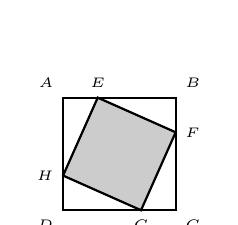
\begin{tikzpicture}[scale=0.55]
      \coordinate (A) at (0,2.6);
      \coordinate (B) at (2.6,2.6);
      \coordinate (C) at (2.6,0);
      \coordinate (D) at (0,0);
      
      \draw[thick] (A) -- (B) -- (C) -- (D) -- cycle;
      \node[above left] at (A) {\tiny $A$};
      \node[above right] at (B) {\tiny $B$};
      \node[below right] at (C) {\tiny $C$};
      \node[below left] at (D) {\tiny $D$};
      
      \coordinate (E) at (0.8,2.6);
      \coordinate (F) at (2.6,1.8);
      \coordinate (G) at (1.8,0);
      \coordinate (H) at (0,0.8);
      
      \fill[gray!40] (E) -- (F) -- (G) -- (H) -- cycle;
      \draw[thick] (E) -- (F) -- (G) -- (H) -- cycle;
      
      \node[above] at (E) {\tiny $E$};
      \node[right] at (F) {\tiny $F$};
      \node[below] at (G) {\tiny $G$};
      \node[left] at (H) {\tiny $H$};
    \end{tikzpicture}
  \end{minipage}

  \item \textbf{(0,5 điểm)} Cho các số thực $a, b$ thỏa mãn $a^2 + b^2 = 2$. Tìm giá trị nhỏ nhất của $P = 3(a + b) + ab$:
  \begin{itemize}[leftmargin=16pt, itemsep=1.5pt, parsep=0pt]
    \item Đặt $t = a + b$. Ta có $t^2 = (a + b)^2 = a^2 + b^2 + 2ab = 2 + 2ab \implies ab = \dfrac{t^2 - 2}{2}$.
    Theo bất đẳng thức Bunhiacopxki: $t^2 = (a + b)^2 \le 2(a^2 + b^2) = 4 \implies -2 \le t \le 2$. \dotfill \textbf{0,15 điểm}
    \item Thay $ab$ vào $P$: $P = 3t + \dfrac{t^2 - 2}{2} = \dfrac{1}{2}t^2 + 3t - 1$. \dotfill \textbf{0,15 điểm}
    \item Biến đổi: $P = \dfrac{1}{2}(t^2 + 6t + 9) - \dfrac{11}{2} = \dfrac{1}{2}(t + 3)^2 - \dfrac{11}{2}$.\\
    Vì $t \in [-2; 2]$ nên $t + 3 \ge 1 > 0$, hàm số đồng biến theo $t$.\\
    Do đó $P$ đạt giá trị nhỏ nhất khi $t = -2$:\\
    $P_{\min} = \dfrac{1}{2}(-2 + 3)^2 - \dfrac{11}{2} = \dfrac{1}{2}(1) - \dfrac{11}{2} = -5$. \dotfill \textbf{0,10 điểm}
    \item Dấu đẳng thức xảy ra khi $\begin{cases} a + b = -2 \\ a^2 + b^2 = 2 \end{cases} \iff a = b = -1$.\\
    Vậy giá trị nhỏ nhất của $P$ là $-5$, đạt được khi $a = b = -1$. \dotfill \textbf{0,10 điểm}
  \end{itemize}
\end{enumerate}

\vspace{2mm}
\hrule
\vspace{2mm}

% --- BẢNG TỔNG HỢP CƠ CẤU ĐIỂM ---
\noindent\textbf{\large BẢNG TỔNG HỢP CƠ CẤU ĐIỂM TOÀN BÀI THI:}
\begin{center}
\small
\renewcommand{\arraystretch}{1.1}
\begin{tabular}{|l|p{11.8cm}|c|}
\hline
\textbf{Phần thi} & \textbf{Nội dung kiến thức đánh giá} & \textbf{Điểm} \\
\hline
\textbf{Phần I} & 8 câu hỏi trắc nghiệm khách quan 4 lựa chọn (0,25đ/câu) & \textbf{2,0 đ} \\
\hline
\textbf{Câu 9} & Phương trình tích (1,0đ) và phương trình chứa ẩn ở mẫu (1,0đ) & \textbf{2,0 đ} \\
\hline
\textbf{Câu 10} & Giải hệ hai phương trình bậc nhất hai ẩn & \textbf{1,0 đ} \\
\hline
\textbf{Câu 11} & Toán thực tế tuyển sinh vào 10 (lập hệ phương trình) & \textbf{1,0 đ} \\
\hline
\textbf{Câu 12} & Toán thực tế chiều cao cái cây (tỉ số lượng giác góc nhọn) & \textbf{1,0 đ} \\
\hline
\textbf{Câu 13} & Hình học tam giác vuông, hệ thức lượng và tam giác đồng dạng & \textbf{2,0 đ} \\
\hline
\textbf{Câu 14} & Cực trị hình học vườn hoa (0,5đ) và GTNN đại số 2 biến (0,5đ) & \textbf{1,0 đ} \\
\hline
\multicolumn{2}{|r|}{\textbf{TỔNG CỘNG TOÀN BÀI THI:}} & \textbf{10,0 đ} \\
\hline
\end{tabular}
\end{center}

\vspace{1mm}
\begin{center}
  \textbf{--- HẾT ---}
\end{center}

\end{document}

